\section{Electrodynamics}
\subsection{Retarded Potentials and Far-Field Radiation (David Tong EM, PS7 Q4)}
\label{sec:retarded-potentials}
Let $\phi$ be the retarded scalar potential given by
\begin{equation}
  \phi(t,\mathbf{x}) = \frac{1}{4\pi\varepsilon_0}\int d^3y\,
  \frac{\rho(t_{\mathrm{ret}},\mathbf{y})}{R},
\end{equation}
where $R = |\mathbf{x}-\mathbf{y}|$, $t_{\mathrm{ret}} = t - R/c$, and
$\hat{\mathbf{R}} = (\mathbf{x}-\mathbf{y})/R$. Show that
\begin{equation}
  \frac{\partial}{\partial t}\phi(t,\mathbf{x})
  = \frac{1}{4\pi\varepsilon_0}\int d^3y\,
  \frac{\dot{\rho}(t_{\mathrm{ret}},\mathbf{y})}{R},
\end{equation}
where $\dot{\rho}(t_{\mathrm{ret}},\mathbf{y})$ is $\partial\rho(t,\mathbf{y})/\partial t$
evaluated at $t_{\mathrm{ret}}$. Show further that
\begin{equation}
  \nabla\phi(t,\mathbf{x}) = -\frac{1}{4\pi\varepsilon_0}\int d^3y\,\hat{\mathbf{R}}
  \left(\frac{1}{R^2}\rho(t_{\mathrm{ret}},\mathbf{y})
  + \frac{1}{cR}\dot{\rho}(t_{\mathrm{ret}},\mathbf{y})\right).
\end{equation}
Hence verify, using $\nabla^2(1/R) = -4\pi\delta^{(3)}(\mathbf{x}-\mathbf{y})$,
that $\phi$ satisfies the wave equation:
\begin{equation}
    \Box\,\phi(t,\mathbf{x}) = -\frac{1}{\varepsilon_0}\rho(t,\mathbf{x}).
\end{equation}

Write down a similar retarded solution for the vector potential $\mathbf{A}$
in terms of the current density $\mathbf{J}$.

Now assume that $\rho$ and $\mathbf{J}$ are non-zero only in a finite region.
Setting $\hat{\mathbf{x}} = \mathbf{x}/|\mathbf{x}|$, show that the leading
terms in the far-field expansion are
\begin{align}
  \mathbf{E}(t,\mathbf{x})
  &\approx \frac{\mu_0}{4\pi|\mathbf{x}|}\int d^3y
    \left(\hat{\mathbf{x}}c\dot{\rho}(t_{\mathrm{ret}},\mathbf{y})
    - \dot{\mathbf{J}}(t_{\mathrm{ret}},\mathbf{y})\right) \notag\\
  &= \frac{\mu_0}{4\pi|\mathbf{x}|}\,\hat{\mathbf{x}}\times
    \left(\hat{\mathbf{x}}\times\int d^3y\,
    \dot{\mathbf{J}}(t_{\mathrm{ret}},\mathbf{y})\right),
\end{align}
where conservation of current, integration by parts, and discarding of a
surface integral have all been used, and
\begin{equation}
  \mathbf{B}(t,\mathbf{x}) \approx -\frac{\mu_0}{4\pi c|\mathbf{x}|}\,
  \hat{\mathbf{x}}\times\int d^3y\,\dot{\mathbf{J}}(t_{\mathrm{ret}},\mathbf{y})
  = \frac{1}{c}\hat{\mathbf{x}}\times\mathbf{E}(t,\mathbf{x}).
\end{equation}
(Note that these results do not assume the dipole approximation.)
Determine the Poynting vector.

\textit{Hint: when using current conservation, and integration by parts, be careful with the $\mathbf{y}$-dependence of $t_{\mathrm{ret}}$.}

\noindent \underline{\textbf{Solution}}
Following from the retarded potential, we have, trivially, 
\begin{equation}
  \frac{\partial}{\partial t}\phi(t,\mathbf{x})
  = \frac{1}{4\pi\varepsilon_0}\int d^3y\,
  \frac{\dot{\rho}(t_{\mathrm{ret}},\mathbf{y})}{R}.
\end{equation}
Then, note that 
\begin{equation}
    \nabla\left(\frac{1}{R}\right) = -\frac{\hat{\mathbf{R}}}{R^2} \qquad \text{and} \qquad \nabla \rho(t_\text{ret},\mathbf{y}) = \frac{\partial\rho(t_\text{ret},\mathbf{y})}{\partial R} = -\frac{1}{c}\dot{\rho}(t_{\mathrm{ret}},\mathbf{y})\hat{\mathbf{R}}.
\end{equation}
Thus, we have
\begin{equation}
    \nabla\phi(t,\mathbf{x}) = -\frac{1}{4\pi\varepsilon_0}\int d^3y\,\hat{\mathbf{R}}
  \left(\frac{1}{R^2}\rho(t_{\mathrm{ret}},\mathbf{y})
  + \frac{1}{cR}\dot{\rho}(t_{\mathrm{ret}},\mathbf{y})\right).
\end{equation}.

Now, first consider the second-order time derivative, which is simply given by
\begin{equation}
    \frac{\partial^2}{\partial t^2}\phi(t,\mathbf{x})
  = \frac{1}{4\pi\varepsilon_0}\int d^3y\,
  \frac{\ddot{\rho}(t_{\mathrm{ret}},\mathbf{y})}{R}.
\end{equation}
For the Laplacian, it is slightly trickier; we find
\begin{equation}
    \nabla^2\phi(t,\mathbf{x}) = -\frac{1}{\varepsilon_0}\rho(t,\mathbf{x}) +\frac{1}{4\pi\varepsilon_0c^2}\int d^3y\,
  \frac{\ddot{\rho}(t_{\mathrm{ret}},\mathbf{y})}{R}.
\end{equation}
Putting them together, we obtain
\begin{equation}
    \square\phi(t,\mathbf{x}) = -\frac{1}{\varepsilon_0}\rho(t,\mathbf{x}).
\end{equation}

By simple analogy, we have
\begin{equation}
    \square\mathbf{A}(t,\mathbf{x}) = -\mu_0\mathbf{J}(t,\mathbf{x}),
\end{equation}
\begin{equation}
    \frac{\partial}{\partial t}\mathbf{A}(t,\mathbf{x})
  = \frac{\mu_0}{4\pi}\int d^3y\,
  \frac{\dot{\mathbf{J}}(t_{\mathrm{ret}},\mathbf{y})}{R},
\end{equation}
and
\begin{equation}
    \nabla A_i(t,\mathbf{x}) = -\frac{\mu_0}{4\pi}\int d^3y\,\hat{\mathbf{R}}
  \left(\frac{1}{R^2}J_i(t_{\mathrm{ret}},\mathbf{y})
  + \frac{1}{cR}\dot{J_i}(t_{\mathrm{ret}},\mathbf{y})\right)
\end{equation}

In the far-field, we have $R\gg 1$ and $|\mathbf{x}|\approx R$, which gives
\begin{align}
    \mathbf{E}(t,\mathbf{x}) &= -\nabla\phi(t,\mathbf{x})-\frac{\partial\mathbf{A}(t,\mathbf{x})}{\partial t}\\
    &\approx\frac{1}{4\pi\varepsilon_0}\int d^3y\,\hat{\mathbf{x}}
  \frac{1}{c|\mathbf{x}|}\dot{\rho}(t_{\mathrm{ret}},\mathbf{y}) - \frac{\mu_0}{4\pi}\int d^3y\,\hat{\mathbf{x}}
  \frac{1}{|\mathbf{x}|}\dot{J_i}(t_{\mathrm{ret}},\mathbf{y})\\
  &=\frac{\mu_0}{4\pi|\mathbf{x}|}\int d^3y
    \left(\hat{\mathbf{x}}c\dot{\rho}(t_{\mathrm{ret}},\mathbf{y})
    - \dot{\mathbf{J}}(t_{\mathrm{ret}},\mathbf{y})\right).
\end{align}

To simplify the first term, consider the continuity equation,
\begin{equation}
    \dot{\rho}(t_\textbf{ret},\mathbf{y}) + \nabla_y\cdot \mathbf{J}(t,\mathbf{y})\bigg|_{t=t_\text{ret}}=0.
\end{equation}
However, to perform an integration by parts, we need
\begin{equation}
    \nabla_y\cdot\mathbf{J}(t_\text{ret},\mathbf{y}) = \nabla_y\cdot \mathbf{J}(t,\mathbf{y})\bigg|_{t=t_\text{ret}} + \dot{\mathbf{J}}(t_\text{ret},\mathbf{y})\cdot\nabla t_\text{ret} = \nabla_y\cdot \mathbf{J}(t,\mathbf{y})\bigg|_{t=t_\text{ret}} + \dot{\mathbf{J}}(t_\text{ret},\mathbf{y})\cdot\frac{\hat{\mathbf{R}}}{c}.
\end{equation}
Thus, the first term integral becomes
\begin{equation}
    \frac{\mu_0}{4\pi|\mathbf{x}|}\int d^3y\,
    \hat{\mathbf{x}}\dot{\mathbf{J}}(t_\text{ret},\mathbf{y})\cdot\hat{\mathbf{R}} - \frac{\mu_0}{4\pi|\mathbf{x}|}\oint d^2y\,\mathbf{J}(t_\text{ret},\mathbf{y})\cdot \hat{\mathbf{n}}.
\end{equation}
Since $\mathbf{J}$ is bounded, the surface integral vanishes. Therefore, we can write
\begin{equation}
    E(t, \mathbf{x}) \approx \frac{\mu_0}{4\pi|\mathbf{x}|}\int d^3y \left(\hat{\mathbf{x}}(\dot{\mathbf{J}}(t_\text{ret},\mathbf{y})\cdot\hat{\mathbf{R}}) - \dot{\mathbf{J}}(t_\text{ret},\mathbf{y})\right),
\end{equation}
Again, for far-field, we have $\hat{\mathbf{R}} \approx \hat{\mathbf{x}}$. Finally, using the vector identity, we find
\begin{equation}
    \mathbf{E}(t,\mathbf{x})
  \approx \frac{\mu_0}{4\pi|\mathbf{x}|}\,\hat{\mathbf{x}}\times
    \left(\hat{\mathbf{x}}\times\int d^3y\,
    \dot{\mathbf{J}}(t_{\mathrm{ret}},\mathbf{y})\right).
\end{equation}

For the magnetic field, we have
\begin{equation}
    B_i(t,\mathbf{x}) = \epsilon_{ijk}\partial_jA_k \approx -\frac{\mu_0}{4\pi c|\mathbf{x}|}\epsilon_{ijk}\int d^3y\,\hat{\mathbf{x}}_j\dot{J}_k(t,\mathbf{x}),
\end{equation}
where we have made a far-field approximation again. Therefore, we find
\begin{equation}
    \mathbf{B}(t,\mathbf{x}) \approx -\frac{\mu_0}{4\pi c|\mathbf{x}|}\,
  \hat{\mathbf{x}}\times\int d^3y\,\dot{\mathbf{J}}(t_{\mathrm{ret}},\mathbf{y})
  = \frac{1}{c}\hat{\mathbf{x}}\times\mathbf{E}(t,\mathbf{x}).
\end{equation}

The Poynting vector of the radiation is, therefore, given by
\begin{equation}
    \mathbf{S(t,\mathbf{x})} = \frac{1}{\mu_0 c}\mathbf{E}(t,\mathbf{x})\times\left(\hat{\mathbf{x}}\times\mathbf{E}(t,\mathbf{x})\right) = \frac{1}{\mu_0c}[\hat{\mathbf{x}}|\mathbf{E}(t,\mathbf{x})|^2 - \mathbf{E}(t,\mathbf{x})(\hat{\mathbf{x}}\cdot\mathbf{E}(t,\mathbf{x}))].
\end{equation}
Note that $\hat{\mathbf{x}}\cdot\mathbf{E}=0$, and hence we have
\begin{equation}
    \mathbf{S(t,\mathbf{x})}=\frac{\mu_0}{16\pi^2c|\hat{\mathbf{x}}|^2}\left|\int d^3y\dot{\mathbf{J}}(t_{\mathrm{ret}},\mathbf{y})\right|^2\sin^2\theta \,\hat{\mathbf{x}},
\end{equation}
where $\theta$ is the angle between the integral and $\hat{\mathbf{x}}$.

\subsection{Liénard--Wiechert Potential and the Field Tensor (David Tong EM, PS7 Q6)}
\label{sec:lienard-wiechert}

For a relativistic particle of charge $q$ on a trajectory
$y^\mu(\tau)$, where $\tau$ is proper time, the current density 4-vector is
\begin{equation}
  J^\mu(x) = qc\int d\tau\,\delta^{(4)}(x-y(\tau))\dot{y}^\mu(\tau),
\end{equation}
with $\dot{y}^\mu\dot{y}_\mu = -c^2$ and $\dot{y}^0 > 0$. Show that the
4-vector potential is given by
\begin{align}
  A^\mu(x)
  &= \frac{\mu_0}{2\pi}\int d^4z\,
     \Theta(x^0-z^0)\,\delta\!\left(\eta_{\alpha\beta}
     (x^\alpha-z^\alpha)(x^\beta-z^\beta)\right)J^\mu(z) \notag\\
  &= -\frac{\mu_0 qc}{4\pi}
     \frac{\dot{y}^\mu(\tau^*)}{R^\nu(\tau^*)\dot{y}_\nu(\tau^*)},
\end{align}
where $R^\nu(\tau) = x^\nu - y^\nu(\tau)$ and $\tau^*$ is determined by
$R^\mu(\tau^*)R_\mu(\tau^*) = 0$ and $R^0(\tau^*) > 0$.

Verify that the Lorenz gauge condition $\partial_\mu A^\mu = 0$ holds and
show that
\begin{equation}
  F^{\mu\nu} = -\frac{\mu_0 qc}{4\pi}
  \frac{1}{(R^\rho\dot{y}_\rho)^2}
  \left(R^\mu S^\nu - R^\nu S^\mu\right),
\end{equation}
where
\begin{equation}
  S^\nu = \ddot{y}^\nu
  - \frac{\dot{y}^\nu}{R^\rho\dot{y}_\rho}\!\left(c^2 + R^\tau\ddot{y}_\tau\right)
\end{equation}
and all quantities on the right are evaluated at $\tau_*$. Check this result
for the case of a stationary charge at the origin.

\noindent \underline{\textbf{Solution}} Given the 4-potential satisfies
\begin{equation}
    \square A^\mu(x) = -\mu_0J^\mu(x).
\end{equation}
To solve this, we shall first find the retarded Green's function of the d'Alembert equation, which satisfies
\begin{equation}
    \square G^{\mu\nu}(x,z) = \delta^{(4)}(x-z)\eta^{\mu\nu}.
\end{equation}
In the Fourier domain, we have
\begin{equation}
    -k^2\tilde{G}^{\mu\nu}(k) = \eta^{\mu\nu}.
\end{equation}
Implementing the retarded prescription, we have
\begin{align}
    G^{\mu\nu}(x,0) &= -\eta^{\mu\nu}\int\frac{d^3\mathbf{k}}{(2\pi)^3}\int\frac{dk^0}{2\pi}\frac{e^{ik^0x^0-i\mathbf{k}\cdot \mathbf{x}}}{(k^0-i\epsilon)^2-|\mathbf{k}|^2}\\
    &= -\eta^{\mu\nu}\Theta(x^0)\int\frac{d^3\mathbf{k}}{(2\pi)^3\cdot 2|\mathbf{k}|}ie^{-i\mathbf{k}\cdot \mathbf{x}}\left[e^{i|\mathbf{k}|x^0}-e^{-i|\mathbf{k}|x^0}\right]\\
    &=\eta^{\mu\nu}\Theta(x^0)\int\frac{d^3\mathbf{k}}{(2\pi)^3|\mathbf{k}|}e^{-i\mathbf{k}\cdot \mathbf{x}}\sin\left(|\mathbf{k}|x^0\right)\\
    &= \frac{\eta^{\mu\nu}}{2\pi^2|\mathbf{x}|}\Theta(x^0)\int^\infty_0d|\mathbf{k}|\sin\left(|\mathbf{k}|x^0\right)\sin\left(|\mathbf{k}||\mathbf{x}|\right)\\
    &= \frac{\eta^{\mu\nu}}{4\pi^2|\mathbf{x}|}\Theta(x^0) \int^\infty_0d|\mathbf{k}|\left[\cos\!\left(|\mathbf{k}|(x^0 - |\mathbf{x}|)\right) - \cos\!\left(|\mathbf{k}|(x^0 + |\mathbf{x}|)\right)\right]\\
    &= \frac{\eta^{\mu\nu}}{4\pi^2|\mathbf{x}|}\Theta(x^0)\cdot\pi\left[\delta(x^0 - |\mathbf{x}|) - \delta(x^0 + |\mathbf{x}|)\right]\\
    &= \frac{\eta^{\mu\nu}}{4\pi|\mathbf{x}|}\Theta(x^0)\,\delta(x^0 - |\mathbf{x}|),
\end{align}
where we used $\int_0^\infty d|\mathbf{k}|\cos(|\mathbf{k}|a) = \pi\delta(a)$, and the second delta function vanishes under $\Theta(x^0)$ since $x^0 + |\mathbf{x}| > 0$ always. Using $\Theta(x^0)\delta(x^2) = \Theta(x^0)\delta(x^0-|\mathbf{x}|)/(2|\mathbf{x}|)$, we obtain
\begin{equation}
    \boxed{G^{\mu\nu}_{\mathrm{ret}}(x,0) = \frac{\eta^{\mu\nu}}{2\pi}\Theta(x^0)\,\delta(x^2).}
\end{equation}
Therefore, the covariant retarded potential can be written as
\begin{equation}
    A^\mu(x) =\frac{\mu_0}{2\pi}\int d^4z\,
     \Theta(x^0-z^0)\,\delta\!\left(\eta_{\alpha\beta}
     (x^\alpha-z^\alpha)(x^\beta-z^\beta)\right)J^\mu(z).
\end{equation}
Using the Dirac delta identities, we can simplify this:
\begin{align}
        A^\mu(x) &= \frac{\mu_0qc}{2\pi}\int d\tau\int d^4z\,
     \Theta(x^0-z^0)\,\delta\!\left(\eta_{\alpha\beta}
     (x^\alpha-z^\alpha)(x^\beta-z^\beta)\right)\delta^{(4)}(z-y(\tau))\dot{y}^\mu(\tau) \notag \\
     &=\frac{\mu_0qc}{2\pi}\int d\tau
     \Theta(x^0-y^0(\tau))\,\delta\!\left(R^\nu(\tau)R_\nu(\tau)\right)\dot{y}^\mu(\tau) \notag\\
     &=\frac{\mu_0qc}{4\pi}\int d\tau
     \Theta(x^0-y^0(\tau))\sum_i\frac{\delta(\tau-\tau_i)}{|R^\nu(\tau_i)\dot{y}_\nu(\tau_i)|}\dot{y}^\mu(\tau),
\end{align}
where $\tau_i$ satisfy $R^\nu(\tau_i)R_\nu(\tau_i) = 0$. The Heaviside function discards all solutions in the future light cone of the point, $x^\mu$. Meanwhile, for any physical object ($v<c$), the trajectory can only cross the past light cone once. Thus, there is only one solution, $\tau_i = \tau^*$.

\begin{figure}[htbp]
\centering
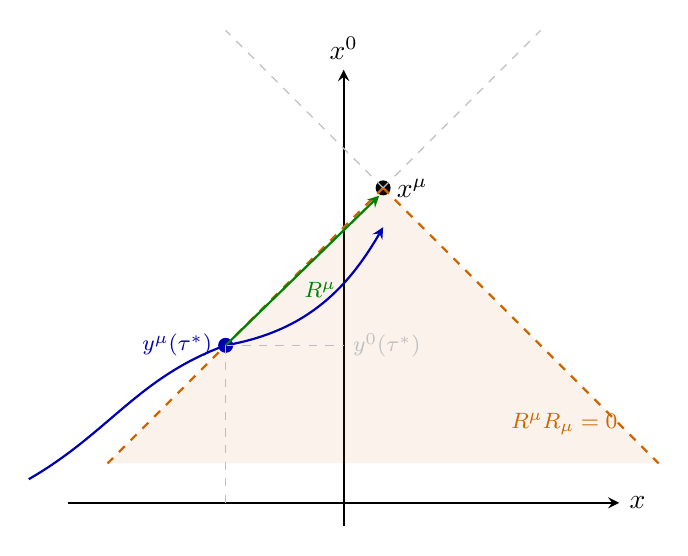
\begin{tikzpicture}

  %% Axes
  \draw[-stealth, thick] (-3.5,0) -- (3.5,0) node[right] {$x$};
  \draw[-stealth, thick] (0,-0.3) -- (0,5.5) node[above] {$x^0$};

  %% Field point x^mu
  \filldraw[black] (0.5, 4) circle (2.5pt);
  \node[right] at (0.55, 4) {$x^\mu$};

  %% Past light cone (going downward from x^mu)
  \draw[thick, dashed, orange!80!black]
    (0.5, 4) -- (-3.0, 0.5) node[left, font=\footnotesize] {};
  \draw[thick, dashed, orange!80!black]
    (0.5, 4) -- (4.0, 0.5);
  \node[orange!80!black, font=\footnotesize] at (2.8, 1.0)
    {$R^\mu R_\mu = 0$};

  %% Shaded past light cone
  \fill[orange!80!black, opacity=0.08]
    (0.5,4) -- (-3.0, 0.5) -- (4.0, 0.5) -- cycle;

  %% Future light cone (going upward, faint)
  \draw[gray!50, dashed, thin]
    (0.5,4) -- (-1.5, 6);
  \draw[gray!50, dashed, thin]
    (0.5,4) -- (2.5, 6);

%% Worldline
  \draw[blue!70!black, thick, -stealth]
    (-4.0, 0.3) to[out=30, in=200] (-1.5, 2.0)
                to[out=10, in=240] (0.5, 3.5);

  %% Intersection tau*
  \filldraw[blue!70!black] (-1.5, 2.0) circle (2.5pt);
  \node[left, blue!70!black, font=\footnotesize] at (-1.55, 2.0)
    {$y^\mu(\tau^*)$};

  %% Dashed lines to axes
  \draw[gray!50, very thin, dashed]
    (-1.5, 2.0) -- (-1.5, 0);
  \draw[gray!50, very thin, dashed]
    (-1.5, 2.0) -- (0, 2.0)
    node[right, font=\footnotesize] {$y^0(\tau^*)$};

  %% R^mu vector
  \draw[-stealth, green!50!black, thick]
    (-1.5, 2.0) -- (0.45, 3.9);
  \node[green!50!black, font=\footnotesize] at (-0.3, 2.7)
    {$R^\mu$};


\end{tikzpicture}
\caption{The worldline $y^\mu(\tau)$ (blue) has slope steeper than $45^\circ$
($v < c$), so it pierces the past light cone of $x^\mu$ exactly once at
$\tau^*$. The $\Theta(x^0 - y^0)$ factor discards intersections with the
future cone. $R^\mu(\tau^*)$ is the resulting null vector.}
\label{fig:lightcone}
\end{figure}

Since $R^\nu(\tau^*)$ is light-like and $\dot{y}^\nu(\tau^*)$ is time-like, $R^\nu(\tau^*)\dot{y}_\nu(\tau^*)<0$. Therefore, we obtain
\begin{equation}
    A^\mu(x) = -\frac{\mu_0qc}{4\pi}\frac{\dot{y}^\mu(\tau^*)}{R^\nu(\tau^*)\dot{y}_\nu(\tau^*)}.
\end{equation}

Now, let us verify that the potential indeed satisfies the Lorenz gauge. First, recall that 
\begin{equation}
    R^\nu(\tau^*)R_\nu(\tau^*) = 0,
\end{equation}
which implies 
\begin{equation}
    \partial_\mu\left(R^\nu(\tau^*)R_\nu(\tau^*)\right) = 2R^\nu(\tau^*)\partial_\mu R_\nu(\tau^*) = 2R^\nu(\tau^*)(\eta_{\mu\nu} - \dot{y}_\nu(\tau^*)\partial_\mu\tau^*)=0.
    \label{eq:pR}
\end{equation}
Thus, we can write $\partial_\mu\tau^*$ in terms of $R$ and $\dot{y}$:
\begin{equation}
    \partial_\mu\tau^* = \frac{R_\mu(\tau^*)}{R^\nu(\tau^*)\dot{y}_\nu(\tau^*)}.
    \label{eq:ptau}
\end{equation}
Then, consider
\begin{equation}
    \partial_\mu A^\mu(x) \propto \partial_\mu\left(\frac{\dot{y}^\mu(\tau^*)}{R^\nu(\tau^*)\dot{y}_\nu(\tau^*)}\right) = \frac{(\partial_\mu \dot{y}^\mu)R^\nu\dot{y}_\nu -  \dot{y}^\mu(\partial_\mu R^\nu)\dot{y}_\nu -  \dot{y}^\mu R^\nu(\partial_\mu\dot{y}_\nu)}{(R^\rho\dot{y}_\rho)^2},
\end{equation}
where we have been a bit sloppy with the notations and dropped the $\tau^*$ in the second equality. The first term in the numerator can be simplified using (\ref{eq:ptau}):
\begin{equation}
    (\partial_\mu \dot{y}^\mu)R^\nu\dot{y}_\nu = (\partial_\mu\tau^*)\ddot{y}^\mu R^\nu\dot{y}_\nu = \ddot{y}^\mu R_\mu.
\end{equation}
Similarly, the third term becomes
\begin{equation}
    -\dot{y}^\mu R^\nu(\partial_\mu\dot{y}_\nu) = - \ddot{y}^\mu R_\mu,
\end{equation}
which cancels the first term. We are left with the second term; using (\ref{eq:pR}), we find
\begin{equation}
    -\dot{y}^\mu(\partial_\mu R^\nu)\dot{y}_\nu= \dot{y}^\mu(\delta_\mu^\nu - \dot{y}^\nu\partial_\mu\tau^*)\dot{y}_\nu = 0,
\end{equation}
where we have used $\dot{y}^\mu\dot{y}_\mu = -c^2$ in the last step. Since all of the terms in the numerator cancel, we have demonstrated that the potential indeed satisfies the Lorenz gauge.

To evaluate the field strength tensor, we use the similar approach as above. Consider
\begin{align}
    \partial^\mu A^\nu  &= -\frac{\mu_0 qc}{4\pi}\frac{1}{(R^\rho\dot{y}_\rho)^2}\left[(\partial^\mu \dot{y}^\nu)R^\tau\dot{y}_\tau -  \dot{y}^\nu(\partial^\mu R^\tau)\dot{y}_\tau -  \dot{y}^\nu R^\tau(\partial^\mu\dot{y}_\tau)\right] \notag
    \\
    &= -\frac{\mu_0 qc}{4\pi}\frac{1}{(R^\rho\dot{y}_\rho)^2}\left[\ddot{y}^\nu R^\mu -  \dot{y}^\nu\dot{y}^\mu - \frac{c^2\dot{y}^\nu  R^\mu}{R^\rho \dot{y}_\rho}-  \frac{\dot{y}^\nu R^\tau\ddot{y}_\tau R^\mu}{R^\rho \dot{y}_\rho}\right].
\end{align}
Thus, we have
\begin{align}
    F^{\mu\nu} &= \partial^\mu A^\nu - \partial^\nu A^\mu= -\frac{\mu_0 qc}{4\pi}\frac{1}{(R^\rho\dot{y}_\rho)^2}\left[\ddot{y}^\nu - \frac{c^2\dot{y}^\nu }{R^\rho \dot{y}_\rho}-  \frac{\dot{y}^\nu R^\tau\ddot{y}_\tau }{R^\rho \dot{y}_\rho}\right]R^\mu - (\mu\leftrightarrow\nu)   \notag \\
    &=-\frac{\mu_0 qc}{4\pi}
  \frac{1}{(R^\rho\dot{y}_\rho)^2}
  \left(R^\mu S^\nu - R^\nu S^\mu\right)
\end{align}
as expected.

For a stationary charge at the origin, we have
\begin{equation}
    y^\mu(\tau) = (c\tau ,0,0,0), \quad \dot{y}^\mu=(c,0,0,0), \quad \text{and}\quad \ddot{y}^\mu = (0,0,0,0).
\end{equation}
Then, 
\begin{equation}
    R^\mu(\tau^*) = (x^0-c\tau^*,\mathbf{x}).
\end{equation}
Using $R^\mu(\tau^*)R_\mu(\tau^*)=0$, we find
\begin{equation}
    (x^0-c\tau^*)^2 = |\mathbf{x}|^2,
\end{equation}
which, in turn, gives
\begin{equation}
    R^\mu(\tau^*)\dot{y}_\mu(\tau^*) = -c|\mathbf{x}|, \quad \text{and} \quad S^\mu = -\left(\frac{c^2}{|\mathbf{x}|},0,0,0\right).
\end{equation}
Finally, we find
\begin{equation}
    \boxed{F^{\mu\nu}=\frac{\mu_0 qc^2}{4\pi |\mathbf{x}|^3}\begin{pmatrix}
    0   & -^1 & -x^2 & -x^3 \\
    x^1 & 0   & 0   & 0   \\
    x^2 & 0   & 0   & 0   \\
    x^3 & 0   & 0   & 0
  \end{pmatrix} = \frac{1}{c}\begin{pmatrix}
    0   & -E^1 & -E^2 & -E^3 \\
    E^1 & 0   & 0   & 0   \\
    E^2 & 0   & 0   & 0   \\
    E^3 & 0   & 0   & 0
  \end{pmatrix}}
\end{equation}
as expected for a stationary charge at the origin since the beginning of time, where
\begin{equation}
    \mathbf{E} = \frac{q\mathbf{x}}{4\pi \varepsilon_0|\mathbf{x}|^3}.
\end{equation}

\subsection{Relativistic Motion in a Uniform Electric Field (David Tong EM, PS3 Q9)}
\label{sec:relativistic-electric}

A particle of rest mass $m$ and charge $q$ moves in a constant
uniform electric field $\mathbf{E} = (E,0,0)$. It starts from the origin with
initial momentum $\mathbf{p} = (0,p_0,0)$. Show that the particle traces out
a path in the $(x,y)$ plane given by
\begin{equation}
  x = \frac{\mathcal{E}_0}{qE}\left(\cosh\!\left(\frac{qEy}{p_0 c}\right)-1\right),
\end{equation}
where $\mathcal{E}_0 = \sqrt{p_0^2c^2 + m^2c^4}$ is the initial kinetic energy
of the particle.

\noindent \underline{\textbf{Solution}} We start with the covariant form of the Lorentz force:
\begin{equation}
    m\frac{dU^\mu}{d\tau} = qF^{\mu\nu}U_\nu.
\end{equation}
Given $U^\mu = (\gamma c, \mathbf{p})$, it becomes
\begin{equation}
    \frac{d\mathbf{p}}{dt} = q\mathbf{E},
\end{equation}
where $\mathbf{p}$ is the relativistic 3-momentum, namely $\mathbf{p} = \gamma m \dot{\mathbf{x}}$. Thus, we can write
\begin{equation}
    \frac{d\mathbf{x}}{dt} = \frac{\mathbf{p}}{\gamma m} = \frac{\mathbf{p}c^2}{\mathcal{E}}.
\end{equation}
This gives
\begin{equation}
    \begin{cases}
        \dot{x} = \dfrac{p_xc^2}{\sqrt{\mathcal{E}_0^2+p_x^2c^2}},\\
        \\
        \dot{y} = \dfrac{p_0c^2}{\sqrt{\mathcal{E}_0^2+p_x^2c^2}}.
        
    \end{cases}
    \label{eq:2}
\end{equation}
Since we can easily solve for $p_x = qEt$, we can solve the two equations and find
\begin{equation}
     y = \frac{p_0c}{eE}\sinh^{-1}\left(\frac{cqEt}{\mathcal{E}_0}\right),
\end{equation}
and
\begin{equation}
    x = \frac{c}{qE}\left(\sqrt{\mathcal{E}_0^2+q^2E^2t^2c^2}-\mathcal{E}_0\right).
\end{equation}
Putting these together, we find
\begin{equation}
    x = \frac{\mathcal{E}_0}{qE}\left(\cosh\!\left(\frac{qEy}{p_0 c}\right)-1\right).
\end{equation}
\begin{figure}[htbp]
\centering
\begin{tikzpicture}
\begin{axis}[
  width=16cm, height=8cm,
  xmin=-0.2, xmax=8,
  ymin=-0.2, ymax=3,
  axis lines=center,
  xtick=\empty,
  ytick=\empty,
  xlabel={$x$},
  ylabel={$y$},
  every axis x label/.style={at={(ticklabel* cs:1.02)}, anchor=west},
  every axis y label/.style={at={(ticklabel* cs:1.05)}, anchor=south},
  clip=false,
]

%% Trajectory: x = cosh(y) - 1, y >= 0
\addplot[black, thick, domain=0:2.8, samples=300]
  ({cosh(x)-1}, {x});

%% Arrow on trajectory at y=1.4
\addplot[-stealth, black, thick, domain=1.39:1.41, samples=5]
  ({cosh(x)-1}, {x});

%% Starting point
\addplot[mark=*, mark size=2.5pt, black] coordinates {(0,0)};

%% Initial momentum arrow
\draw[-stealth, thick] (axis cs:0,0) -- (axis cs:0,0.6)
  node[left, font=\footnotesize] {$\mathbf{p}_0$};

%% Electric field arrow
\draw[-stealth, thick] (axis cs:1.5,2.5) -- (axis cs:2.2,2.5)
  node[right, font=\footnotesize] {$\mathbf{E}$};

\end{axis}
\end{tikzpicture}
\caption{Trajectory of a relativistic charged particle in a uniform electric
field $\mathbf{E}=(E,0,0)$, in natural units $\mathcal{E}_0/qE = p_0c/qE = 1$.
The particle starts at the origin with momentum $\mathbf{p}_0$ in the
$y$-direction and follows $x = (\mathcal{E}_0/qE)(\cosh(qEy/p_0c)-1)$.}
\label{fig:catenary}
\end{figure}

\subsection{Gauge Transformation of a Plane Electromagnetic Wave (David Tong EM, PS3 Q5)}
\label{sec:gauge-plane-wave}

Consider a plane polarized electromagnetic wave described by the
vector and scalar potentials,
\begin{equation}
  \mathbf{A}(\mathbf{r},t) = \mathbf{A}_0\,e^{i(\mathbf{k}\cdot\mathbf{r}-\omega t)}
  \qquad\text{and}\qquad
  \phi(\mathbf{r},t) = \phi_0\,e^{i(\mathbf{k}\cdot\mathbf{r}-\omega t)},
\end{equation}
with constant $\mathbf{A}_0$ and $\phi_0$. Use Maxwell's equations to find a
relationship between $\mathbf{A}_0$ and $\phi_0$.

Find a gauge transformation such that the new vector potential is
``transversely polarised'', i.e.\ $\mathbf{A}_0\cdot\mathbf{k}=0$ (Coulomb
gauge, $\nabla\cdot\mathbf{A}=0$). What is the scalar potential $\phi$ in
this gauge?

\noindent \underline{\textbf{Solution}} The Maxwell equations give
\begin{equation}
    \nabla^2\phi +\frac{\partial}{\partial t}\nabla\cdot \mathbf{A} =0,
\end{equation}
and
\begin{equation}
    \nabla\times(\nabla\times\mathbf{A}) = -\frac{1}{c^2}\left[\nabla\left(\frac{\partial \phi}{\partial t}\right) + \frac{\partial^2\mathbf{A}}{\partial t^2}\right] = \nabla(\nabla\cdot \mathbf{A})-\nabla^2\mathbf{A}.
\end{equation}
Then, we find
\begin{equation}
    \mathbf{k}^2 \phi_0 - \omega\mathbf{k}\cdot \mathbf{A}_0 = 0.
\end{equation}

If we set the Coulomb gauge, we find
\begin{equation}
    \phi_0 = 0.
\end{equation}

\subsection{Reflection of an Electromagnetic Wave from a Moving Mirror (David Tong EM, PS3 Q7)}
\label{sec:moving-mirror}

An electromagnetic wave is reflected by a perfect conductor at
$x=0$. The electric field has the form
\begin{equation}
  \mathbf{E}(t,\mathbf{x}) = \hat{\mathbf{y}}\left[f(t_-) - f(t_+)\right],
    \label{eq:E}
\end{equation}
where $f$ is an arbitrary function and $ct_\pm = ct\pm x$. Show that this
satisfies the relevant boundary condition at the conductor. Find the
corresponding magnetic field $\mathbf{B}$.

Show that under a Lorentz transformation to a frame moving with speed $v$ in
the $x$-direction, the electric field is transformed to
\begin{equation}
  \mathbf{E}'(t',\mathbf{x}') = \hat{\mathbf{y}}\left[
    \rho f(\rho t'_-) - \frac{1}{\rho}f\!\left(\frac{t'_+}{\rho}\right)
  \right],
  \qquad\text{where}\quad
  \rho = \sqrt{\frac{c-v}{c+v}}\,.
\end{equation}

Hence for an incident wave $\mathbf{E}(t,\mathbf{x}) = \hat{\mathbf{y}}F(t_-)$,
find the wave that is reflected after it hits a perfectly conducting mirror
moving with speed $v$ in the $x$-direction.

\noindent \underline{\textbf{Solution}} It is clear to see that the electric field of this form has an ingoing part, $f(t_-)$, and an outgoing part, $f(t_+)$. The boundary condition at a perfect conductor is given by 
\begin{equation}
    \hat{\mathbf{x}}\cdot (\mathbf{E}_+- \mathbf{E}_-) = \frac{\sigma}{\varepsilon_0} = 0, \quad \text{and}\quad \hat{\mathbf{x}}\times(\mathbf{E}_+- \mathbf{E}_-) =0.
\end{equation}
It is clear to see that (\ref{eq:E}) satisfies the boundary condition. To find the magnetic field, let's first take the curl of the electric field, which gives
\begin{align}
    \nabla \times \mathbf{E} &= -\hat{\mathbf{y}} \times[\nabla f(t_-) - \nabla f(t_+)] = \frac{\hat{\mathbf{y}}\times \hat{\mathbf{x}}}{c}[\dot{f}(t_-) + \dot{f}(t_+)]= -\frac{\hat{\mathbf{z}}}{c}[\dot{f}(t_-) + \dot{f}(t_+)].
\end{align}
Hence, the magnetic field is given by
\begin{equation}
    \mathbf{B}(t,\mathbf{x}) = \frac{\hat{\mathbf{z}}}{c} [f(t_-) + f(t_+)].
\end{equation}

For a boost in the $x$-direction, the electric field transforms like
\begin{equation}
    E_x'= E_x, \quad E_y' = \gamma(E_y-vB_z),\quad \text{and}\quad E_z'=\gamma(E_z+vB_y).
\end{equation}
Therefore, we have
\begin{equation}
    \mathbf{E}'(t',\mathbf{x}') = \gamma[f(t_-)-f(t_+)]\hat{\mathbf{y}}-\frac{v}{c}\gamma[f(t_-)+f(t_+)]\hat{\mathbf{y}} = \hat{\mathbf{y}}[\rho f(t_-) -\frac{1}{\rho}f(t_+)].
\end{equation}
Now, we express the coordinates in the primed coordinates, which is
\begin{equation}
    ct_\pm = \gamma\left(ct'+\frac{vx'}{c^2}\pm x' \pm vt'\right) = \frac{\gamma}{c}\left[(c\pm v)t' \pm(c\pm v)x'\right]=\begin{cases}
        \rho t_-',\\
        \dfrac{1}{\rho}t_+'.
    \end{cases}
\end{equation}
Thus, we find
\begin{equation}
  \mathbf{E}'(t',\mathbf{x}') = \hat{\mathbf{y}}\left[
    \rho f(\rho t'_-) - \frac{1}{\rho}f\!\left(\frac{t'_+}{\rho}\right)
  \right].
\end{equation}

In the frame where the mirror is stationary, the incident electric field is given by $\hat{\mathbf{y}}\rho F(\rho t_-')$. Since the mirror is stationary in this frame, the reflected electric field must be $-\hat{\mathbf{y}}\rho F(\rho t_+')$. Given the transformation law we just derived, the reflected electric field in the rest frame is $-\hat{\mathbf{y}}\rho^2 F(\rho^2 t_+)$. The total electric field is given by
\begin{equation}
    \mathbf{E}(t,\mathbf{x}) = \hat{\mathbf{y}}\left[F(t_-) -\rho^2 F(\rho^2 t_+) \right].
\end{equation}


\subsection{Covariant Form of Ohm's Law (David Tong EM, PS3 Q10)}
\label{sec:ohm-covariant}

For a general 4-velocity, written as $u^\mu = \gamma(c,\mathbf{v})$,
show that
\begin{equation}
  F_{\mu\nu}u^\nu = \gamma\begin{pmatrix}-\mathbf{E}\cdot\mathbf{v}/c\\[4pt]
  \mathbf{E}+\mathbf{v}\times\mathbf{B}\end{pmatrix}.
\end{equation}

In the rest-frame of a conducting medium, Ohm's law states that
$\mathbf{J}=\sigma\mathbf{E}$, where $\sigma$ is the conductivity and
$\mathbf{J}$ is the 3-current. Assuming that $\sigma$ is a Lorentz scalar,
show that Ohm's law can be written covariantly as
\begin{equation}
  J^\mu + \frac{1}{c^2}(J^\nu u_\nu)u^\mu = \sigma F^{\mu\nu}u_\nu,
\end{equation}
where $J^\mu$ is the 4-current and $u^\mu$ is the (uniform) 4-velocity of
the medium. If the medium moves with 3-velocity $\mathbf{v}$ in some inertial
frame, show that the current in that frame is
\begin{equation}
  \mathbf{J} = \rho\mathbf{v} + \sigma\gamma\!\left(\mathbf{E}
  + \mathbf{v}\times\mathbf{B} - \frac{1}{c^2}(\mathbf{v}\cdot\mathbf{E})\mathbf{v}\right),
\end{equation}
where $\rho$ is the charge density. Simplify this formula, given that the
charge density vanishes in the rest-frame of the medium.

\noindent \underline{\textbf{Solution}} It is easy to verify that 
\begin{equation}
    F_{\mu\nu}u^\nu = \gamma\begin{pmatrix}
  0        &  E_x/c &  E_y/c &  E_z/c \\
  -E_x/c  &  0     & -B_z   &  B_y   \\
  -E_y/c  &  B_z   &  0     & -B_x   \\
  -E_z/c  & -B_y   &  B_x   &  0
\end{pmatrix}
\begin{pmatrix}
    c\\v_x\\v_y\\v_z
\end{pmatrix} = 
   \gamma\begin{pmatrix}-\mathbf{E}\cdot\mathbf{v}/c\\
  \mathbf{E}+\mathbf{v}\times\mathbf{B}\end{pmatrix}.
\end{equation}

In the rest-frame, $u^\mu = (c,0,0,0)$. Then, consider
\begin{equation}
    J^\mu + \frac{1}{c^2}(J^\nu u_\nu)u^\mu = \begin{pmatrix}
        \rho c\\\mathbf{J}
    \end{pmatrix}+\frac{1}{c^2}\begin{pmatrix}
        -\rho c &\mathbf{J}
    \end{pmatrix}\cdot\begin{pmatrix}
        c\\0
    \end{pmatrix}\begin{pmatrix}
        c\\0
    \end{pmatrix} = \begin{pmatrix}
        0\\\mathbf{J}
    \end{pmatrix},
\end{equation}
and
\begin{equation}
    \sigma F_{\mu\nu}u^\nu = \begin{pmatrix}
        0\\\sigma\mathbf{E}.
    \end{pmatrix}
\end{equation}
Thus, we have verified that 
\begin{equation}
  J^\mu + \frac{1}{c^2}(J^\nu u_\nu)u^\mu = \sigma F^{\mu\nu}u_\nu
\end{equation}
is indeed the covariant representation of Ohm's law.

For a moving medium, the equation gives
\begin{equation}
    \begin{pmatrix}
        \rho c+\gamma^2(-\rho c^2+\mathbf{J}\cdot\mathbf{v})\\
        \mathbf{J} +\gamma^2(-\rho c^2+\mathbf{J}\cdot\mathbf{v})\mathbf{v}/c
    \end{pmatrix}  =\gamma \sigma\begin{pmatrix}
        \mathbf{E}\cdot\mathbf{v}/c\\\mathbf{E}+\mathbf{v}\times\mathbf{B} \end{pmatrix}.
\end{equation}
Combining the two equations, we find
\begin{equation}
    \mathbf{J} = \rho\mathbf{v} + \sigma\gamma\!\left(\mathbf{E}
  + \mathbf{v}\times\mathbf{B} - \frac{1}{c^2}(\mathbf{v}\cdot\mathbf{E})\mathbf{v}\right).
\end{equation}

Finally, given $\rho_0 = 0$, then $J^\mu u_\mu = -\rho_0 c^2$. This implies
\begin{equation}
    -\rho c^2 + \mathbf{J}\cdot\mathbf{v} = 0,
\end{equation}
Taking the dot product of $\mathbf{J}$
with $\mathbf{v}$ gives
\begin{equation}
    \rho v^2 + \sigma\gamma\left(\mathbf{v}\cdot\mathbf{E} - \frac{v^2}{c^2}\mathbf{v}\cdot\mathbf{E}\right)
    = \rho c^2.
\end{equation}
Rearranging, we find
\begin{equation}
    \rho = \frac{\sigma \gamma}{c^2}\,\mathbf{v}\cdot\mathbf{E}.
\end{equation}
Substituting back, the current becomes
\begin{equation}
    \mathbf{J}
    = \sigma\gamma\left(\mathbf{E}+\mathbf{v}\times\mathbf{B}\right).
\end{equation}

\subsection{Dielectric Sphere in a Uniform Electric Field (David Tong EM, PS8 Q1)}
\label{sec:dielectric-sphere}

A dielectric sphere of radius $a$ and permittivity $\varepsilon$ is
placed at rest at the origin in a constant electric field which takes a uniform
value $\mathbf{E}_0$ far from the origin. Show that Maxwell's equations with
the appropriate boundary conditions are solved by an electric field which is
uniform inside the sphere, with value:
\begin{equation}
  \mathbf{E}_{\mathrm{int}} = \frac{3}{2+\varepsilon_r}\mathbf{E}_0,
\end{equation}
where $\varepsilon_r = \varepsilon/\varepsilon_0$, and a field outside the
sphere which is the superposition of $\mathbf{E}_0$ and the field
\begin{equation}
  \mathbf{E}(\mathbf{x}) = \frac{1}{4\pi\varepsilon_0}
  \left(\frac{3(\mathbf{p}\cdot\hat{\mathbf{x}})\hat{\mathbf{x}}-\mathbf{p}}{|\mathbf{x}|^3}\right)
\end{equation}
of an electric dipole at the origin, with dipole moment
\begin{equation}
  \mathbf{p} = 4\pi\varepsilon_0\!\left(\frac{\varepsilon_r-1}{\varepsilon_r+2}\right)a^3\mathbf{E}_0.
\end{equation}

By considering the macroscopic polarisation $\mathbf{P}$ inside the sphere,
calculate the bound surface charge density $\sigma$. Verify explicitly that
the electric dipole moment of $\sigma$ is $\mathbf{p}$.

\noindent \underline{\textbf{Solution}} Inside and outside the dielectric, the potential satisfies the Laplace equation,
\begin{equation}
    \nabla^2\phi = 0.
\end{equation}
Since the problem is invariant under rotation about $\mathbf{E}_0$, which we will take to be in the $z$-direction, the solution should have no $\phi$ dependence. Then, the general solution for the Laplace equation is 
\begin{equation}
    \phi(r,\theta) =  \sum_{l=0}^\infty (A_lr^{l} + B_lr^{-(l+1)})P_l(\cos\theta).
\end{equation}
Inside the dielectric, we require regularity at the origin; we set $B_l =0$. Outside the dielectric, since there is a constant electric field at $\mathbf{E}_0 = E_0\cos\theta\hat{\mathbf{z}}$ $r\to\infty $, we take $A_l = -E_0\delta_{l1}$. So the general solution we are looking at is
\begin{equation}
    \phi(r,\theta)  = \begin{cases}
        \displaystyle\sum_{l=0}^\infty A_lr^lP_l(\cos\theta),&r<a,\\
        \\\displaystyle\sum_{l=0}^\infty D_lr^{-(l+1)}P_l(\cos\theta) -E_0r\cos\theta,&r>a.
    \end{cases}
\end{equation}
The boundary condition at $r=a$ is given by
\begin{equation}
    \hat{\mathbf{r}}\times(\mathbf{E}(a\hat{\mathbf{r}}^+)-\mathbf{E}(a\hat{\mathbf{r}}^-)) = 0,\quad \text{and} \quad \hat{\mathbf{r}}\cdot(\varepsilon_0\mathbf{E}(a\hat{\mathbf{r}}^+)-\varepsilon\mathbf{E}(a\hat{\mathbf{r}}^-)) = 0,
\end{equation}
which implies
\begin{equation}
    \partial_\theta\phi(a^+,\theta) = \partial_\theta\phi(a^-,\theta), \quad \text{and} \quad \varepsilon_0\partial_r\phi(a^+,\theta) = \varepsilon\partial_r\phi(a^-,\theta).
\end{equation}
The first BC gives
\begin{equation}
    A_la^l = D_la^{-(l+1)}-E_0a\delta_{l1},
\end{equation}
and the second BC gives
\begin{equation}
    \varepsilon_0lA_la^{l-1} =-\varepsilon(l+1)D_la^{-(l+2)}-\varepsilon E_0\delta_{l1}.
\end{equation}
Solving these two, we find
\begin{equation}
    A_l = -\frac{3}{2+\varepsilon_r}E_0 \delta_{l1}\quad\text{and} \quad D_1 = -\frac{1-\varepsilon_r}{2+\varepsilon_r}a^3E_0\delta_{l1}.
\end{equation}
Hence, the full potential is
\begin{equation}
    \phi(r,\theta) = \begin{cases}
        -\dfrac{3}{2+\varepsilon_r}E_0r\cos\theta, & r<a,\\
        -\dfrac{1-\varepsilon_r}{2+\varepsilon_r}\dfrac{a^3}{r^2}E_0\cos\theta-E_0r\cos\theta, & r>a.
    \end{cases}
\end{equation}

Therefore, the electric field inside the dielectric is
\begin{equation}
    \mathbf{E}_{\text{int}} = \frac{3}{2+\varepsilon_r}E_0(\cos\theta\,\hat{\mathbf{r}} - \sin\theta\,\hat{\mathbf{\theta}}) = \frac{3}{2+\varepsilon_r}E_0\hat{\mathbf{x}}.
\end{equation}
The electric field outside is
\begin{equation}
    \mathbf{E}(\mathbf{x}) +\mathbf{E}_0 =\frac{1-\varepsilon_r}{2+\varepsilon_r}a^3\frac{(\mathbf{E}_0\cdot\hat{\mathbf{r}})\mathbf{r}-\mathbf{E}_0}{r^3} + \mathbf{E}_0 =\frac{1}{4\pi\varepsilon_0}
  \left(\frac{3(\mathbf{p}\cdot\hat{\mathbf{x}})\hat{\mathbf{x}}-\mathbf{p}}{|\mathbf{x}|^3}\right) + \mathbf{E}_0
\end{equation}
with
\begin{equation}
  \mathbf{p} = 4\pi\varepsilon_0\!\left(\frac{\varepsilon_r-1}{\varepsilon_r+2}\right)a^3\mathbf{E}_0.
\end{equation}
A sketch of the electric field is shown in Fig. \ref{fig:dielectric-fieldlines}.
\begin{figure}[htbp]
\centering
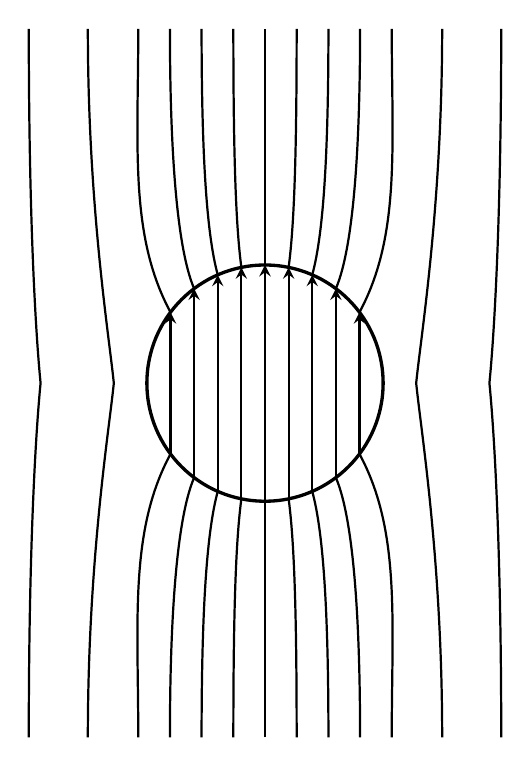
\begin{tikzpicture}[scale=1.5, line width=0.8pt]

%% ====== OUTSIDE FIELD LINES ======

%% Central axial line
\draw (0,-3) -- (0,-1);
\draw (0, 1) -- (0, 3);

%% Entering lines: (x_inf,-3) -> (x_b,-y_b)
%% Control points chosen to match tangent slope of E at sphere boundary
%% x_b=0.2, x_inf=0.268, y_b=0.980
\draw ( 0.268,-3) .. controls ( 0.268,-2.0) and ( 0.250,-1.35) .. ( 0.2,-0.980);
\draw (-0.268,-3) .. controls (-0.268,-2.0) and (-0.250,-1.35) .. (-0.2,-0.980);

%% x_b=0.4, x_inf=0.537, y_b=0.917
\draw ( 0.537,-3) .. controls ( 0.537,-2.0) and ( 0.500,-1.28) .. ( 0.4,-0.917);
\draw (-0.537,-3) .. controls (-0.537,-2.0) and (-0.500,-1.28) .. (-0.4,-0.917);

%% x_b=0.6, x_inf=0.805, y_b=0.800
\draw ( 0.805,-3) .. controls ( 0.805,-2.0) and ( 0.750,-1.15) .. ( 0.6,-0.800);
\draw (-0.805,-3) .. controls (-0.805,-2.0) and (-0.750,-1.15) .. (-0.6,-0.800);

%% x_b=0.8, x_inf=1.073, y_b=0.600
\draw ( 1.073,-3) .. controls ( 1.073,-2.0) and ( 1.150,-1.25) .. ( 0.8,-0.600);
\draw (-1.073,-3) .. controls (-1.073,-2.0) and (-1.150,-1.25) .. (-0.8,-0.600);

%% Exiting lines: (x_b,y_b) -> (x_inf,3)  [symmetric to entering]
\draw ( 0.2, 0.980) .. controls ( 0.250, 1.35) and ( 0.268, 2.0) .. ( 0.268, 3);
\draw (-0.2, 0.980) .. controls (-0.250, 1.35) and (-0.268, 2.0) .. (-0.268, 3);

\draw ( 0.4, 0.917) .. controls ( 0.500, 1.28) and ( 0.537, 2.0) .. ( 0.537, 3);
\draw (-0.4, 0.917) .. controls (-0.500, 1.28) and (-0.537, 2.0) .. (-0.537, 3);

\draw ( 0.6, 0.800) .. controls ( 0.750, 1.15) and ( 0.805, 2.0) .. ( 0.805, 3);
\draw (-0.6, 0.800) .. controls (-0.750, 1.15) and (-0.805, 2.0) .. (-0.805, 3);

\draw ( 0.8, 0.600) .. controls ( 1.150, 1.25) and ( 1.073, 2.0) .. ( 1.073, 3);
\draw (-0.8, 0.600) .. controls (-1.150, 1.25) and (-1.073, 2.0) .. (-1.073, 3);

%% Around-sphere lines: x_inf=1.5, x_equator=1.28
\draw ( 1.5,-3) .. controls ( 1.50,-1.5) and ( 1.32,-0.4) ..
      ( 1.28, 0) .. controls ( 1.32, 0.4) and ( 1.50, 1.5) .. ( 1.5, 3);
\draw (-1.5,-3) .. controls (-1.50,-1.5) and (-1.32,-0.4) ..
      (-1.28, 0) .. controls (-1.32, 0.4) and (-1.50, 1.5) .. (-1.5, 3);

%% x_inf=2.0, x_equator=1.90
\draw ( 2.0,-3) .. controls ( 2.0,-1.0) and ( 1.91,-0.1) ..
      ( 1.90, 0) .. controls ( 1.91, 0.1) and ( 2.0, 1.0) .. ( 2.0, 3);
\draw (-2.0,-3) .. controls (-2.0,-1.0) and (-1.91,-0.1) ..
      (-1.90, 0) .. controls (-1.91, 0.1) and (-2.0, 1.0) .. (-2.0, 3);

%% ====== WHITE FILL — masks outside lines inside sphere ======
\fill[white] (0,0) circle (1);

%% ====== INSIDE FIELD LINES (on top of white fill) ======
%% Arrow at midpoint (y=0) shows upward field direction
\draw (0,-1) -- (0,0);
\draw[-stealth] (0,0) -- (0,1);

\foreach \xv/\yv in {
   0.2/0.980,  0.4/0.917,  0.6/0.800,  0.8/0.600,
  -0.2/0.980, -0.4/0.917, -0.6/0.800, -0.8/0.600}{
  \draw (\xv,-\yv) -- (\xv, 0);
  \draw[-stealth] (\xv, 0) -- (\xv,\yv);
}

%% ====== SPHERE BOUNDARY ======
\draw[line width=1.2pt] (0,0) circle (1);



\end{tikzpicture}
\caption{Electric field lines for a dielectric sphere ($\varepsilon_r=3$, $a=1$)
in a uniform applied field $\mathbf{E}_0$. Inside the field is uniform and
weaker, $\mathbf{E}_{\mathrm{int}}=\frac{3}{5}\mathbf{E}_0$; outside it is
the superposition of $\mathbf{E}_0$ and an electric dipole. Lines refract at
the boundary satisfying continuity of $E_\parallel$ and $D_\perp$.}
\label{fig:dielectric-fieldlines}
\end{figure}
The polarisation vector is given by
\begin{equation}
    \mathbf{P} = (\varepsilon_r-1)\varepsilon_0\mathbf{E}_\text{int}.
\end{equation}
The bound charge density is simply given by
\begin{equation}
    \sigma(\theta)= \hat{\mathbf{r}}\cdot\mathbf{P} = \frac{3(\varepsilon_r-1)}{2+\varepsilon_r}\varepsilon_0E_0\cos\theta.
\end{equation}
The dipole due to the surface charge distribution is, therefore, given by
\begin{equation}
    \mathbf{p} =  \int_{-1}^1 d\cos\theta\,2\pi\sigma(\theta)a^2\cos\theta = 4\pi\varepsilon_0\!\left(\frac{\varepsilon_r-1}{\varepsilon_r+2}\right)a^3\mathbf{E}_0,
\end{equation}
which indeed matches what we obtained by solving the Laplace equation.

\subsection{Frustrated Total Internal Reflection and Evanescent Waves  (David Tong EM, PS8 Q3)}
\label{sec:ftir}

Two plane, semi-infinite dielectric slabs with refractive index $n$ are separated by a vacuum region of width $d$. A plane wave of wavenumber $k$ is incident on the vacuum region from one of the slabs at an angle of incidence $\theta_I$ to the normal, with $n \sin \theta_I > 1$. The electric field of the incident radiation is normal to the plane of incidence (normal polarisation).

Show that some of the radiation is transmitted across the gap, and that the ratio of the amplitudes of the electric fields of the transmitted and incident waves satisfies:
\begin{equation}
\left| \frac{E_T}{E_I} \right|^2 = \frac{1}{1 + \alpha^2 \sinh^2 \kappa d},
\end{equation}
where
\begin{equation}
\alpha = \frac{k(1 - 1/n^2)}{2\kappa \cos \theta_I}
\quad \text{and} \quad
\kappa = k \sqrt{\sin^2 \theta_I - \frac{1}{n^2}}.
\end{equation}
(This process is known as frustrated total internal reflection and is analogous to quantum tunnelling.)

[\textit{Hint: you will need to consider both growing and decaying evanescent waves in the gap since it is of finite width.}]

\noindent \underline{\textbf{Solution}} Let's take the first interface to be at $x=0$, and the incident electric field to be in the $y$-direction.
The electric field of the whole setup can be written as
\begin{equation}
    \mathbf{E}(t, \mathbf{x}) = \hat{\mathbf{y}}\begin{cases}
        E_{I0}e^{i\mathbf{k}_I\cdot \mathbf{x}-i\omega t } + E_{R0}e^{i\mathbf{k}_R\cdot \mathbf{x}-i\omega t },&x<0,\\
        E_{+0}e^{i\mathbf{k}_+\cdot \mathbf{x}-i\omega t } + E_{-0}e^{i\mathbf{k}_-\cdot \mathbf{x}-i\omega t }, &0<x<d,\\
        E_{T0}e^{i\mathbf{k}_T\cdot \mathbf{x}-i\omega t },&   x>d,
    \end{cases}
\end{equation}
where  we take 
\begin{equation}
    \mathbf{k}_I = (k\cos\theta_I,0,-k\sin\theta_I), \quad \mathbf{k}_R=(-k_R\cos\theta_R, 0, -k_R\sin\theta_R),
\end{equation}
\begin{equation}
    \mathbf{k}_+ = (k_+\cos\theta_+,0,-k_+\sin\theta_+), \quad \mathbf{k}_-=(-k_-\cos\theta_-, 0, -k_-\sin\theta_-),
\end{equation}
and
\begin{equation}
    \mathbf{k}_T = (k_T\cos\theta_T,0,-k_T\sin\theta_T).
\end{equation}
At the boundaries, we require
\begin{equation}
    \hat{\mathbf{{x}}}\cdot(\varepsilon_1\mathbf{E}^+ - \varepsilon_0\mathbf{E}^-)=0, 
    \label{eq:E//}
\end{equation}
\begin{equation}
    \hat{\mathbf{{x}}}\times(\mathbf{E}^+ - \mathbf{E}^-)=0, 
    \label{eq:Ep}
\end{equation}
\begin{equation}
    \hat{\mathbf{{x}}}\times(\varepsilon_1\mathbf{B}^+ - \varepsilon_0\mathbf{B}^-)=0,
    \label{eq:Bp}
\end{equation}
\begin{equation}
    \hat{\mathbf{{x}}}\cdot(\mathbf{B}^+ - \mathbf{B}^-)=0.
    \label{eq:B//}
\end{equation}
Hence, the phase factor at the boundary must vanishes for all $t$, $z$, and $y$ for our case. Therefore, all the angular frequencies are set to be the same. The boundary condition also requires
\begin{equation}
    \mathbf{k}_I\cdot \hat{\mathbf{z}} = \mathbf{k}_R\cdot \hat{\mathbf{z}} = \mathbf{k}_+\cdot \hat{\mathbf{z}}= \mathbf{k}_-\cdot \hat{\mathbf{z}}
    \label{eq:con1}
\end{equation}
at $x=0$. (\ref{eq:con1}) tells us that
\begin{equation}
    k\sin\theta_I = k_R\sin\theta_R = k_+\sin\theta_+ = k_-\sin\theta_-.
\end{equation}
In the dielectric, we have
\begin{equation}
    \frac{ck}{n} = \frac{ck_R}{n} = \omega,
\end{equation}
which implies $k=k_R$ and $\theta_I = \theta_R$.
Therefore,
\begin{align}
    \frac{n\omega}{c}\sin\theta_I = k_\pm \sin\theta_\pm  \implies \mathbf{k}_\pm \cdot \hat{\mathbf{x}} &= \pm\sqrt{|\mathbf{k}_\pm|^2 -(\mathbf{k}_\pm \cdot \hat{\mathbf{z}})^2 } \notag\\&=\pm k\sqrt{1/n^2-\sin^2\theta_I} = \pm i\kappa,
\end{align}
which is the evanescent wave in the vacuum due to the total reflection ($n\sin\theta_I >1$).

The electric field can be rewritten as 
\begin{equation}
    \mathbf{E}(\mathbf{x}) = \hat{\mathbf{y}}\begin{cases}
        E_{I0}e^{i\mathbf{k}_I\cdot \mathbf{x} } + E_{R0}e^{i\mathbf{k}_R\cdot {\mathbf{x}} },&x<0,\\
        E_{+0}e^{i\mathbf{k}_I\cdot \hat{\mathbf{z}} z}e^{-\kappa x} + E_{-0}e^{i\mathbf{k}_I\cdot \hat{\mathbf{z}}z }e^{+\kappa x}, &0<x<d,\\
        E_{T0}e^{i\mathbf{k}_T\cdot \mathbf{x}},&   x>d,
    \end{cases}
\end{equation}
where we have hidden the time-dependence for convenience.
By the same boundary condition at $x=d$, we find
\begin{equation}
    - k_T\sin\theta_T \,z= -k_I\sin\theta_I \,z \implies  \theta_T = \theta_I \quad \text{and} \quad k_I = k_T.
\end{equation}

The corresponding magnetic field is given by
\begin{equation}
\mathbf{B}(\mathbf{x}) = \begin{cases}
\frac{1}{\omega}\Big[
(-k_{Iz}\hat{\mathbf x} + k_{Ix}\hat{\mathbf z}) E_{I0} e^{i\mathbf{k}_I\cdot \mathbf{x}}
+
(-k_{Rz}\hat{\mathbf x} + k_{Rx}\hat{\mathbf z}) E_{R0} e^{i\mathbf{k}_R\cdot \mathbf{x}}
\Big], & x<0, \\[6pt]
\frac{1}{\omega}\Big[
(-k_{Iz}\hat{\mathbf x} + i\kappa \hat{\mathbf z}) E_{+0} e^{i\mathbf{k}_I\cdot \hat{\mathbf z} z} e^{-\kappa x}
+
(-k_{Iz}\hat{\mathbf x} - i\kappa \hat{\mathbf z}) E_{-0} e^{i\mathbf{k}_I\cdot \hat{\mathbf z} z} e^{+\kappa x}
\Big], & 0<x<d, \\[6pt]
\frac{1}{\omega}
(-k_{Tz}\hat{\mathbf x} + k_{Tx}\hat{\mathbf z}) E_{T0} e^{i\mathbf{k}_T\cdot \mathbf{x}}, & x>d.
\end{cases}
\end{equation}

Now, we are left to match the amplitude at the boundaries. By (\ref{eq:E//}), we have
\begin{equation}
    E_{I0} + E_{R0} = E_{+0} + E_{-0},
\end{equation}
and
\begin{equation}
    E_{T0} =E_{+0}e^{-\kappa d} + E_{-0}e^{+\kappa d}.
\end{equation}
Also, by (\ref{eq:B//}), we have
\begin{equation}
    i\kappa(E_{+0}-E_{-0}) = k\cos\theta_I(E_{I0}-E_{R0}),
\end{equation}
and
\begin{equation}
    k\cos\theta_IE_{T0} = i\kappa(E_{+0}e^{-\kappa d}-E_{-0}e^{+\kappa d}).
\end{equation}
With some tedious algebra, one would find
\begin{equation}
\left| \frac{E_T}{E_I} \right|^2 = \frac{1}{1 + \alpha^2 \sinh^2 \kappa d}.
\end{equation}









